In this section, the aim is to predict the performance of the speaker, from his characteristics in terms of training data and speech turns properties. If we are able to predict, reliably, if the $Spkshow$ will be correctly recognized or not, when analysing on the main features contributing to this prediction, we can identify what are the features that  facilitates or hamper the identification, for a given system.

At each $SpkShow$ is associated the maximal $Fm$ obtained accross systems. Doing so, we do not focus on a particular system, but we try to explain "the-best-we-can-do" performance for each $SpkShow$.

\subsection{Detection}


\subsection{Prediction}


\begin{figure}[t]
\centering
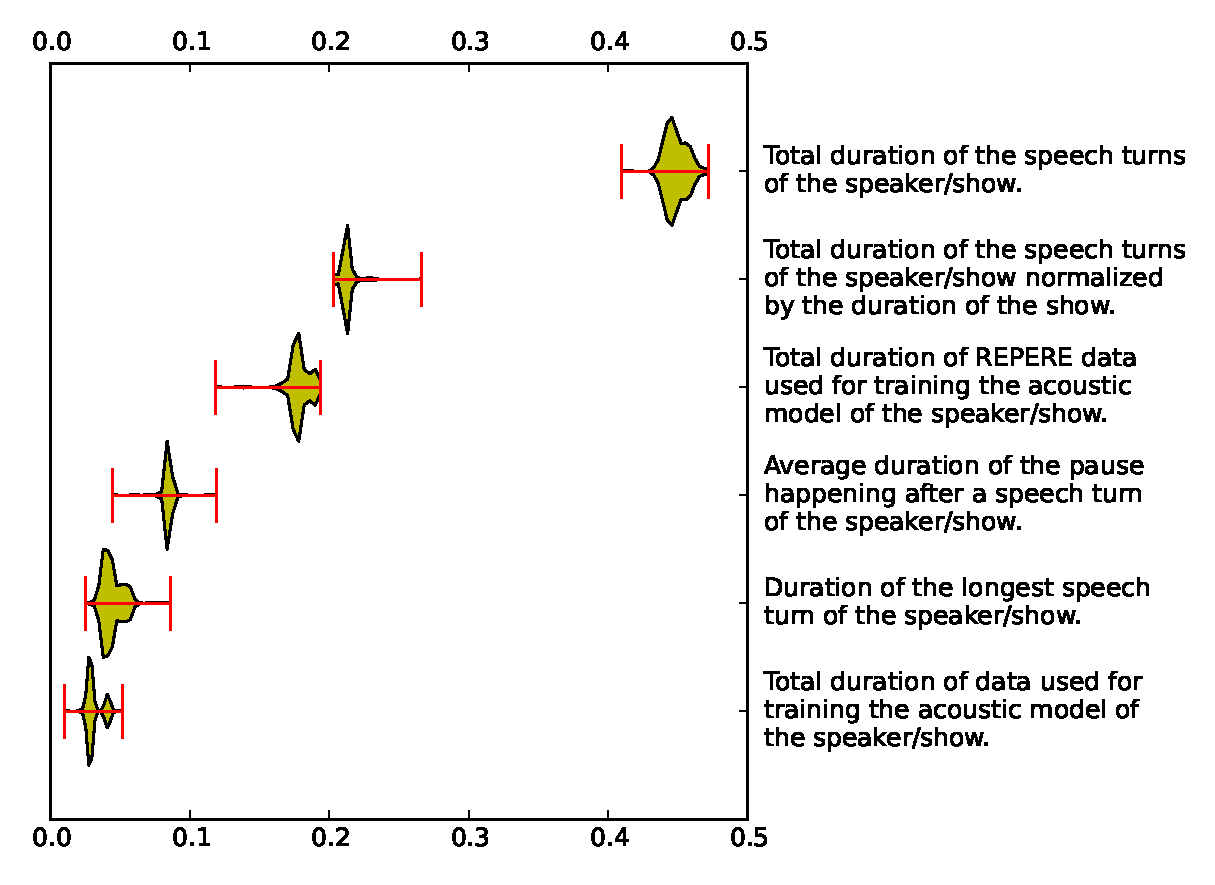
\includegraphics[width=\linewidth]{figures/violin.eps}
\caption{Distribution of feature importance.}
\label{fig:featureImportance}
\end{figure}


Feature importance === Gini coefficent~\cite{Breiman2001}


\begin{figure}[t]
\centering
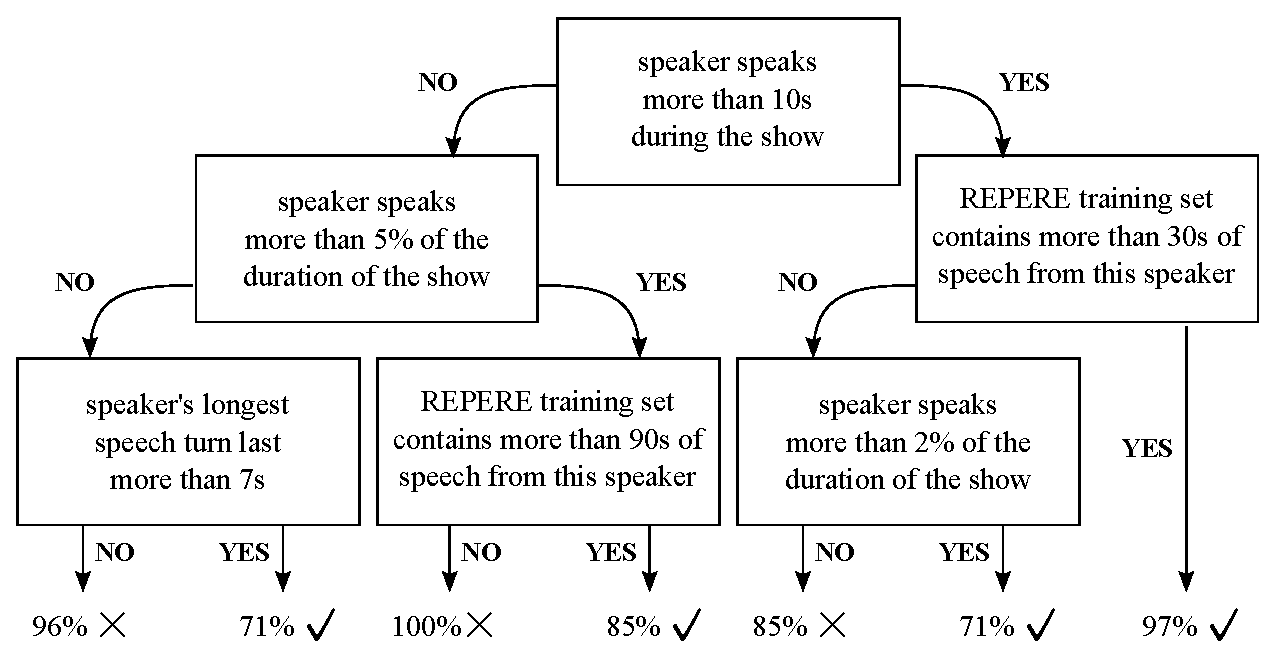
\includegraphics[width=\linewidth]{figures/tree.eps}
\caption{Not recognized ($\times$) vs. (partially) recognized ($\checkmark$)}
\label{fig:tree}
\end{figure}
